\documentclass[11pt]{article}
\usepackage{fullpage}
\usepackage{graphicx} % Required for inserting images
\usepackage{amsthm} % For proof symbols
\usepackage{algorithm}
\usepackage{wrapfig}

\title{Developing a BOGO Coin with Fair Coins}
\author{Austin Burgess, Zach Potthoff, Alex Rimerman}
\date{May 6, 2023}

\begin{document}

\maketitle

\section*{Introduction}

\quad In computer science terms, we call a coin to be something that simulates a coin being flipped in 
real life, but instead of heads or tails coming up, we see 0's and 1's. A coin can either be fair 
or a BOGO coin. In the former case, there is an equal chance of either a 1 or a 0 appearing, as 
the value returned from the function is uniformly distributed on the set \{0, 1\}. A BOGO coin, 
on the other hand, is defined to have a non-uniform output on the set \{0, 1\}. In probability terms,
a BOGO coin produces the output 1 with a probability of p, and produce output of 0 with
probability 1 - p, where $p\in(0, 1), p\neq0.5$. This is analogous to a real-life coin being an unfair one. 

The focus of this paper and our recent research will be on developing an algorithm that represents 
a BOGO coin, given a fair coin. Earlier in the semester, in lab, we developed pseudo-code for a 
fair coin algorithm if given an unknown BOGO coin. For our research, we want to do essentially the 
opposite. Given a parameter p, which is the probability of the BOGO coin outputting a 1, our 
algorithm takes a number of fair coins and transforms them into a single BOGO coin, with an output 
that is within a specific error of p. 

The idea behind this algorithm is dependent on how accurate Python's random number generator is.
More specifically in our case, how uniformly it can choose a 0 vs a 1 to produce a fair coin.
In order for us to get the most accurate results it is our assumption that Python is perfectly uniform
over the set \{0, 1\}. Obviously, given that it is randomly choosing, it will not end up that
100 coin flips will always result in 50 1's and 50 0's, but assuming that it is perfectly random allows
us to properly analyze our results and how well our function works.


\subsection*{Related Works$^1$}

\quad As a way of sampling from non-uniform distributions, Markov chain Monte Carlo algorithms 
are often used. They are a grouping of algorithms that go through a step-by-step process while 
recording the states of specified steps. In essence, these algorithms are taking samples from 
known distributions, and then proceed to use those samples as a way of developing the desired 
distribution. As one may be able to infer even from this brief description, with more steps come 
more accurate results in terms of a distribution.

For the purposes of our research, we did not go much further into Markov chain Monte 
Carlo algorithms than what was just described. We used our understanding of these algorithms at 
a high level to help develop our ideas in creating an algorithm for a BOGO coin while sampling 
from a number of fair coins. At a high level, this seems analogous to the idea of Markov chain 
Monte Carlo algorithms because we take a symmetric binomial distribution and turn it into a 
skewed binomial distribution based on the parameter p. Thus, we kept the principle idea of Markov 
chain Monte Carlo algorithms in mind when developing our own algorithm for a BOGO coin.


\section*{Methods}

\quad Given we decided on an implementation project, we started out by mapping the plan of attack for
the code. This was our list of implementation goals in order:

\begin{enumerate}
    \item \textbf{Set up the fair coin function}
        \subitem This was done first because in order for us to create a BOGO coin out of a certain 
        number of fair coin flips, we needed to have the fair coin created already.
    \item \textbf{Get the BOGO coin function to work when p = .25}
        \subitem We did this because it was the easiest p value to calculate before we moved on to the
        more complicated values. We knew that the algorithm we would need to use was not
        too complex, but at the same time would be a good stepping stone for the beginning
    stages of our project.
    \item \textbf{Get the BOGO coin function to work with a certain error probability
    for all hundredths numbers}
        \subitem After coming up with an algorithm that can generate a BOGO coin with p = 0.25, 
        we want to also be able to generate a BOGO coin for any p rounded to the hundredths 
        place. This is slightly more involved, as p is not necessarily as easy of a decimal as 
        0.25, but there are only a finite number of possibilities. So, being able to compute 
        a BOGO coin for any hundredth decimal serves as a bridge between easy and more complex 
        values of p for our BOGO coin to take.
    \item \textbf{Get the BOGO coin function to work with a certain error probability
    for all thousandth numbers}
        \subitem After doing all hundredths, the natural progression was to do all the thousandths.
        It is a little more complicated than the hundredths but not severely. As we said in the
        description of doing hundredths, doing thousandths was a continuation of us bridging to
        all the possible numbers that we could set p too. 
    \item \textbf{Get the BOGO coin function to work when p = 1/3}
        \subitem This serves as a step towards very complicated BOGO coins. Since we are able to 
        compute all truncated decimals to the thousandths, we want to look into decimals that 
        continue on for many levels of precision (or infinite in this case).
    \item \textbf{Get the BOGO coin function to work with a certain error probability
    for all rational numbers}
        \subitem This goal was considered to be somewhat of a stretch and unknown to us in 
        planning if we would get to it. We want to be able to take a decimal of any length that 
        is rational and be able to compute it within a certain error probability. This is a big 
        step as it allows us to generate a BOGO coin that has very few restrictions in terms of 
        accuracy.
    \item \textbf{Get the BOGO coin function to work with a certain error probability
    for all numbers}
        \subitem At the start of our project, this seemed like a stretch goal. We wanted to see
        if we could get anywhere close to an accurate representation of a p-value like 1/$\pi$.
        Naturally, this was our last goal because if we could make our BOGO coin represent
        an approximation of all numbers, then we have done our original assignment, which was
        to make a BOGO coin that works for any p.
\end{enumerate} 

\subsection*{Developing the Algorithm}
    \quad As outlined in our goals for the project, we wanted to begin by attempting to build the 
    algorithm for p-values that were easy to work with. A major factor that must be considered when 
    using any coin is that there are only two outcomes: a 0 or a 1 being returned. So, probabilities 
    that are in terms of clean powers of $\frac{1}{2}$ will be much easier to find. So, since we did 
    not want to use $p=.5$ as that would be a fair coin, we decided to start with the next simplest 
    p-value: .25. 

    This was done by flipping two fair coins. In this case, flipping two fair coins provides 
    us with 4 distinct and uniform solutions: \{(0, 0), (0, 1), (1, 0), (1, 1)\}. We chose (1, 1) to 
    represent heads for the BOGO coin, allowing for heads to only appear on average 1/4 of the time. 
    We then flipped the BOGO coin 1000 times, and determined what our $\hat{p}$ value would be for 
    these 1000 flips. We then repeated this 1000 times and plotted the results to see if our value was 
    accurate. We will discuss the results in the results section. This algorithm, while fairly simple, 
    was able to provide us with some good insight on what we were going to need to do as we moved 
    to the more complicated p-values.

    As we moved on in our goals of the project, we needed to get more specific with the p-values. One thing 
    that we noticed almost immediately was that 2 fair coins were unable to accurately generate a BOGO coin 
    whose p-value was not 0.00, 0.25, 0.50, 0.75, or 1.00. The reasoning for this flaw was quite obvious: 
    we hard-coded what we wanted p to be by saying how many of the 4 coin pairs were considered a "success," 
    and thus what the probability of flipping a success is. Our algorithm was not yet taking any parameter p.
    Rather, we were picking how many of the 4 pairs of fair coin flips were considered a success, and saying 
    that was our success probability. Realizing this led us to another flaw in the algorithm as it was 
    too reliant on perfectly clean values of p in order generate our BOGO coin. It required that we have 
    an integer for a constant c satisfying the following equation:
    \begin{center}
        $p = \frac{c}{4} = \frac{c}{2^2}, 0.00 \leq p \leq 1.00$
    \end{center}

    If c took the value of a decimal, the algorithm did not work and we could not accurately compute p. 
    This makes logical sense as c represents the number of pairs that are considered a success for our 
    BOGO coin. Since it would not make sense to have $c = 1.5$ successful pairs of numbers, our algorithm 
    would not make much sense. 
    
    THEOREM 1: In the worst case, with our given algorithm, it is possible for error up to $\epsilon = 0.125$.

    \begin{proof} If we want a BOGO coin to take on $p = 0.125$, given we only have 4 fair coins and our 
    current algorithm, we must select either 0 pairs or 1 pair of fair coins selected as successes. If we let 
    X be an indicator random variable of whether a 1 was flipped or not, we see that the expected value is not 
    the same as p. In the two cases:
    \begin{enumerate}
        \item \textbf{0 pairs are considered successes}
        
        $E(X) = 0.00 \neq 0.125 = p$

        $\epsilon = |p - E(X)| = |0.125 - 0.00| = 0.125$

        \item \textbf{1 pair is considered a success}

        $E(X) = 0.25 \neq 0.125 = p$

        $\epsilon = |p - E(X)| = |0.125 - 0.25| = 0.125$     
    \end{enumerate}

    Since the two errors are equal, this is the maximum error if we are trying to minimize error in our generation of 
    a BOGO coin as it is exactly halfway between 0 and 0.25.
    \end{proof}

    With this proof, we can see that the error is at most $\frac{1}{2^{n+1}}$ where n is the number of coins used. So, 
    in order to decrease error in our approximation, we saw that we need to increase the number of coins used. Since our 
    error is $O((\frac{1}{2})^n)$, increasing the number of coins exponentially decreases the error. 
    
    So, we know we have 
    to increase the number of coins to get a closer approximation of p, but we cannot realistically hard-code that many pairs 
    of fair coin combinations. However, we are able to flip an arbitrarily large number of fair coins, assigning a bit value
    to each flip. This gives every possible value in the set $\{0, 1,..., 2^n-1\}$ an equal chance of occurring. From this, we
    are able to take a parameter p and multiply it by $2^n$. This serves as a cutoff for our new and improved algorithm because 
    approximately (due to rounding) p of the possible values (all with equal chance of occurring) in the set are less than the cutoff, 
    while approximately 1-p of the values in the set are larger than the cutoff. Therefore, if the value generated from the 
    fair coin bits is less than our cutoff, we return a 1 as that is the probability of a success. Otherwise, we return 0. 
    And, as we saw, the error will be at most $\frac{1}{2^{n+1}}$ for n fair coins flipped.

    The following psedocode outlines our algorithm if 10 coins are used:

    \begin{algorithm}
        \caption{BOGO Coin}
        \textbf{Parameter} - \textit{p}: the desired probability of success of the coin
        
        \vspace{4mm}
        \textit{numCoins} $\leftarrow 10$

        \textit{coins} $\leftarrow$ initialize empty list

        \textit{cutoff} $\leftarrow p * 2^{numCoins}$

        \textit{total} $\leftarrow 0$

        \textbf{for} every coin
        
        \hspace{3mm}
        Flip a fair coin, append the result to \textit{coins}

        \textbf{end for}

        \textbf{for} i in $0:numCoins$

        \hspace{3mm}
        $total += coins[i] * 2^i$

        \textbf{end for}

        \textbf{if} $total <$ \textit{cutoff}

        \hspace{3mm}
        \textbf{return 1}
        
        \textbf{end if}

        \textbf{return 0}
    \end{algorithm}


\section*{Results}

\quad We determined that the best way to represent our results would be through histograms, plotting
the distribution of the different p values that were gained by different BOGO coin flips. Essentially, we
used our BOGO coin algorithm to represent one BOGO coin flip with probability heads of p. We then would flip
this coin anywhere from 1,000 to 100,000 to show one sample of what p could be, by dividing number of heads
by number of flips to represent our $\hat{p}$ for the given sample. We would repeat this sampling 1,000 times
in order to create a distribution and compare it to what the actual p value should be.

The first graph I will show is our original algorithm of 2 coins to make p = .25. In this graph and all of
our graphs that follow, the black line is what p should actually be, and the green line is our $\hat{p}$ 
value that was determined using the algorithm explained above.

\begin{figure}[h]
    \caption
    \centering
    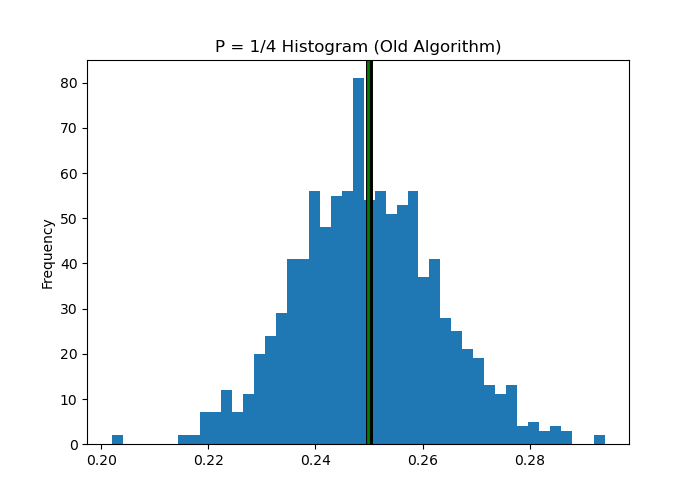
\includegraphics[width=8.5cm, height=4.7cm]{25-1000-old.png}
    \centering
\end{figure}


In Figure 1, we see that the p value we wanted was .25. Our distribution showed that our average $\hat{p}$
was 0.24973. This graph represents p = .25 using 2 fair coin flips per BOGO coin flip, 1,000 BOGO coin flips
per sample, and 1,000 samples. This is a very close to accurate representation of p = .25, as we were about
.00027 off. Because .25 is an exact power of $\frac{1}{2}$, this slight error we determined is due to the 
randomness of the fair coin. While it should be a 50/50 pick, the outcomes will not always be 50/50.

We can compare this graph to a graph of the same p = .25, but now with 10 fair coin flips per BOGO coin flip, 
1,000 BOGO coin flips per sample, and 1,000 samples:

\begin{figure}[h]
    \caption
    \centering
    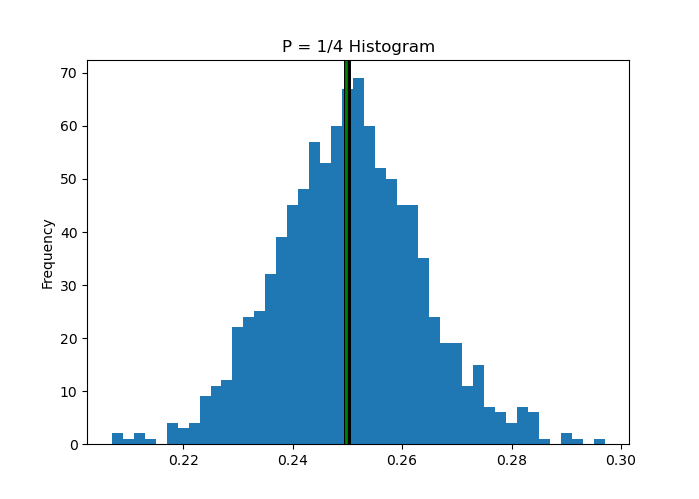
\includegraphics[width=8.5cm, height=4.7cm]{fourth1000.png}
    \centering
\end{figure}

In Figure 2 $\hat{p}$ was .24983. We can see in this distribution that the more fair coin flips per BOGO 
flip led us to a similar looking normal distribution. The use of more coins did not change much of anything
because p was .25. There is a perfect integer c that satisfies both p = $\frac{c}{4}$ and p = $\frac{c}{1024}$.
We will continue the use of this 10 coin strategy with more complex numbers because as stated earlier, there
will be less expected error for numbers that do not have this perfect c.

Next, we have our hundredths example. We wanted to represent .83 using 10 fair coin flips per BOGO coin flip, 
10,000 BOGO coin flips per sample, and 1,000 samples:


\begin{figure}[h]
    \caption
    \centering
    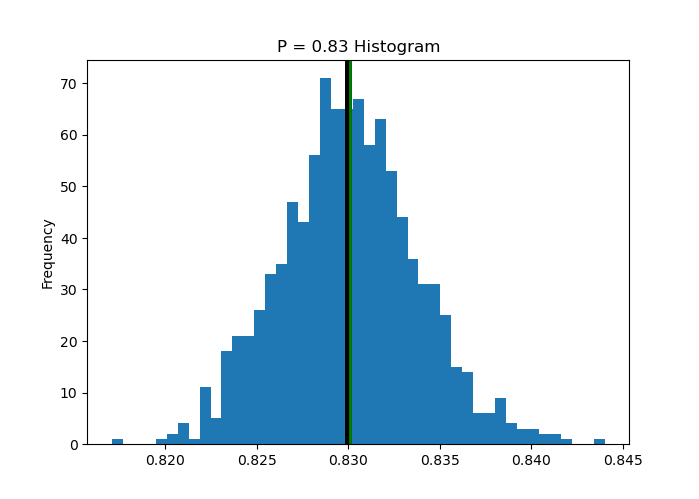
\includegraphics[width=8.5cm, height=5cm]{83-10000.png}
    \centering
\end{figure}

In Figure 3, our distribution led to $\hat{p}$ of .8300712. We can see that this is .0000712 away from our
actual p value. Using 10 fair coin flips per BOGO coin flip allows us to get all numbers with error at most
$\frac{1}{{2}^{11}}$. This led to us having a fairly easy time getting numbers close to any specific 
hundredths value, since 1/2048 is .000488.

Our next goal was to work with a number in the thousandths. We chose p = .181, and we continued with using 
10 fair coin flips per BOGO coin flip, 10,000 BOGO coin flips per sample, and 1,000 samples:

\begin{figure}[h]
    \caption
    \centering
    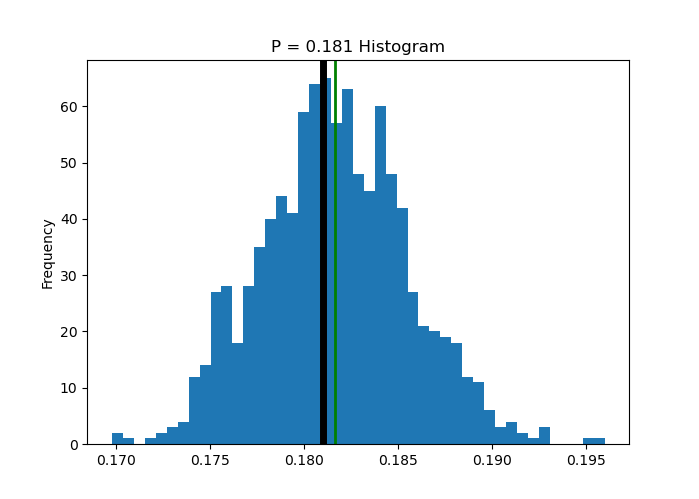
\includegraphics[width=8.5cm, height=5cm]{181-10000.png}
    \centering
\end{figure}

Based on Figure 4, our $\hat{p}$ was determined to be .181652, which is seen to be .000652 away from
our goal p value. Again, this is probably most likely due to the randomness of the fair coin, but with
so many coin flips, a minuscule decimal away makes a lot of sense.

Our last non-stretch goal was to obtain p of 1/3. We decided to increase the number of fair coins per
BOGO coin flip to 100. This will allow our error to be extremely low, as we can now cover a lot more
ground in terms of individual p values that could be more specific decimals. However, due to Python's
randomness, it still will not be perfect. We also are continuing to use 10,000 BOGO coin flips per sample,
and 1,000 samples:

\begin{figure}[h]
    \caption
    \centering
    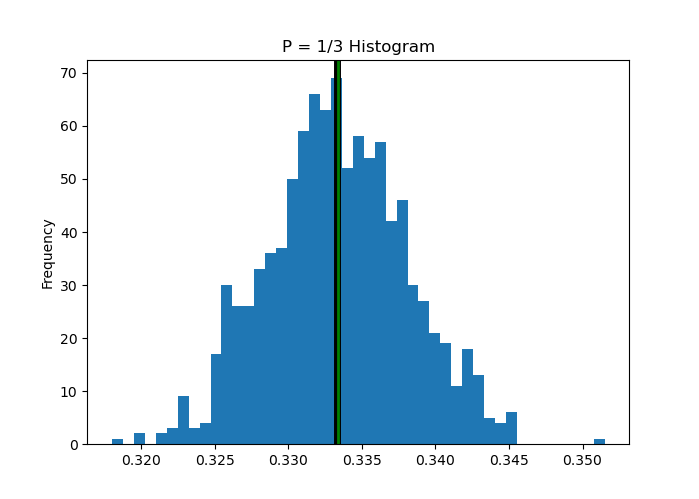
\includegraphics[width=8.5cm, height=5cm]{33-100coins.png}
    \centering
\end{figure}

In Figure 5, we obtained a $\hat{p}$ of .333351. This is approximately .000018 away from our desired
result. The increasing of our number of fair coins was extremely beneficial in providing tighter bounds 
for our $\hat{p}$ value, giving us a much better approximation of p for our program.

We were successful in our first stretch goal of generating a BOGO coin for a p value of any rational number 
between 0 and 1. We chose to try for p = .62531. We continued using 100 fair coin flips per BOGO coin flip, 
10,000 BOGO coin flips per sample, and 1,000 samples:

\begin{figure}[h]
    \caption
    \centering
    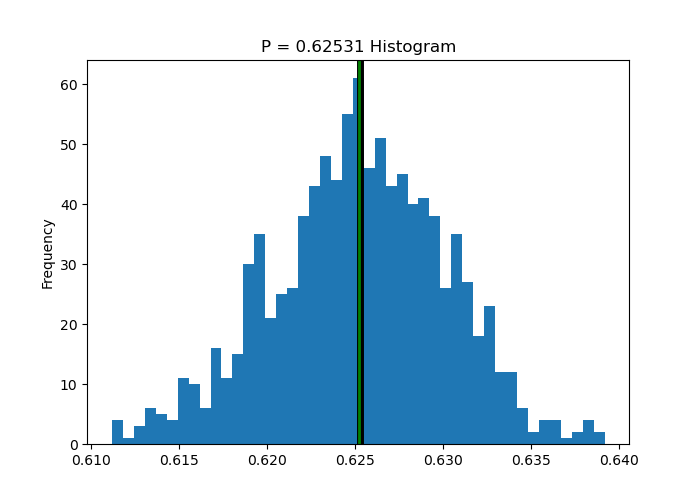
\includegraphics[width=8.5cm, height=5cm]{6253-100coins.png}
    \centering
\end{figure}

We can see in Figure 6 that our $\hat{p}$ was .6252618. This is .0000482 away from the p value
that we were shooting for. This was interesting to see that we were able to obtain a value this close
to our desire p because originally we did not think we would be able to do this for such a long decimal.

Lastly, we decided to see if we could make a BOGO coin that worked for an irrational value of p. We
tried it on 1/$\pi$. Again we used 100 fair coin flips per BOGO coin flip, 10,000 BOGO coin flips per sample, 
and 1,000 samples:

\begin{figure}[h]
    \caption
    \centering
    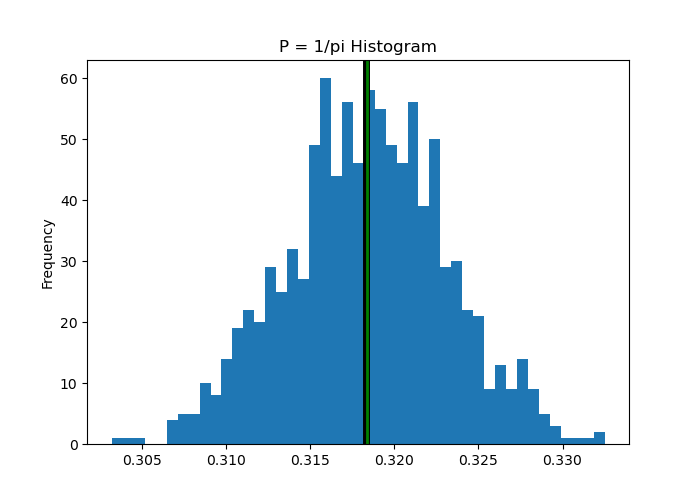
\includegraphics[width=8.5cm, height=5cm]{100coins.png}
    \centering
\end{figure}

\vspace{2cm}
Figure 7 produced a $\hat{p}$ of .318347. 1/$\pi$ is approximately .318309 but obviously continues further
as it is an irrational number. Our $\hat{p}$ value was around .000038 away from the intended target. We were
extremely happy with this because this seemed to us like a close enough estimate that it could be used to
represent 1/$\pi$. Again, due to the randomness of fair coin, there is bound to be some sort of slight
error with $\hat{p}$, but we were able to reduce the significance of this error by increasing the number
of fair coins per BOGO coin flip.

\section*{Discussion and Conclusion}
\quad After executing our algorithm, we can see a clear improvement between 2, 10, and 100 coins. As we 
increase the number of coins, the difference between $\hat{p}$ and the parameter p grows smaller. Although, we do not see a 
perfect amount of error reduction as 100 coins does not guarantee a difference of $O(\frac{1}{2^{101}})$.
Rather, that is the maximum error between the parameter p and the expected value of p that our algorithm 
outputs. This error does not account for extraneous factors such as the randomness of flipping any coin a 
number of times as well as the potential for imperfect randomness with any programming language. However, 
as we increase the number of coin flips, the bounds still get tighter because the standard deviation of 
our estimate goes down (as we are working with a binomial distribution where $\sigma_{\hat{p}}=\sqrt{\frac{p*(1-p)}{n}}$).

Going back to our theorem from earlier, we can further generalize the error to any number of coins. 
We saw that the error will be at most $\frac{1}{2^{n+1}}$ for n fair coins being flipped. Additionally,
looking at our prior equation $p = \frac{c}{4}$ for 2 fair coins, we can generalize this further to say 
that our generated p will be the most accurate when $p=\frac{c}{2^n}, 0.00 \leq p \leq 1.00$ and c is 
an integer. Further generalizing, the error will be at a maximum when c is a decimal with .5 in the 
decimal (for example: 1.5, 2.5, etc.). This was shown in a simpler case in our theorem and proof, as that is the halfway point between 
a perfect estimate of p, and thus where the error is maximized. Combining these two ideas, we see 
that our estimate is more accurate when c is a value which satisfies $p=\frac{c}{2^n}, 0.00 \leq p \leq 1.00$ 
and c is close to an integer. If c is exactly an integer, our expected error will be 0. But, if 
c is a .5 decimal, our expected error will be maximized at $\epsilon = \frac{1}{2^{n+1}}$.

To wrap it up, we were able to achieve all of our goals that we set out for ourselves. Even goals that
we originally had recognized as stretch goals, we were able to accomplish within a certain error.
We consider our project a huge success. It went a lot better than we could have imagined. Once we were
able to develop a strong algorithm for all p values of hundredths decimal place, the rest came naturally.
All we had to do was slightly adjust total fair or BOGO coin flips to allow for less error probability
within our algorithm. We determined that our BOGO coin function could be used as an adequate algorithm to 
simulate a BOGO coin flip for any desired p.

\section*{Acknowledgements}
We would like to thank Professor Joshua Brody for his guidance and assistance in building this project 
as well as Professor Lucas Van Meter for their inspiration for the idea of the project.

\section*{References}
\begin{enumerate}
    \item Wikimedia Foundation. (2023, April 4). Markov chain Monte Carlo. Wikipedia. Retrieved May 3, 2023, from https://en.wikipedia.org/wiki/Markov\_chain\_Monte\_Carlo 
\end{enumerate}

\end{document}
